\section{Functional and Technical Requirements}
\label{sec:requirements}

\subsection{Functional Requirements}
%What function(s) does the subsystem have to fulfill?
%
Below are listed the primary functional requirements for the \ac{EPS}:
%
\begin{itemize}
\item Provide adequate power to motors and payload
\item Proof that flying on solar energy is possible i.e more power produced than consumed
\end{itemize}
%
Additional desired requirements are:
%
\begin{itemize}
\item Scalability to higher power levels
\item Flexible and robust design, allowing flight in more extreme conditions (altitude, weather etc.)
\item Optimal design and high performance to increase power capability and minimize system mass
\end{itemize}
%
%
\subsection{Technical Requirements}
%What technical requirements constrain the subsystem design? - e.g. mass, power, strength, stability etc.
%
The \ac{EPS} technical requirements are listed in table \ref{tab:technical_requirements}.
%
\begin{table}[H]
\centering
\caption{Technical requirements for the \ac{EPS}}
\label{tab:technical_requirements}
\begin{tabular}{p{0.4\textwidth}p{0.4\textwidth}}
\hline
Minimum power output & $8\,W$\\
Maximum mass & $750\,g$(including solar arrays)\\
Maximum cost & $2500\,SEK$\\
Maximum internal power dissipation & $<500\,mW$\\
Output voltages & $3.3\,V$(un-regulated), $5\,V$( regulated)\\
Regulator phase margin & $60\,deg$\\
Regulator gain margin & $10\,dB$\\
Control loop bandwidth & $>10\,kHz$\\
Operational temperature & $-20^{\circ}C\,to +25^{\circ}C$\\
Battery capacity & $>5\,Wh$ ($>30\,min$ of battery powered flight)\\
\hline
\end{tabular}
\end{table}
%
\subsection{Mission and Environmental Constraints}
\label{subsec:environmental_requirements}
This section discusses some of the challenges opposed by the mission and the parameters of operation environment and how these will influence the \ac{EPS} design constraints.
%
\subsubsection*{Solar Array Temperature}
Temperature variation of the solar panels, significantly changes the solar panels characteristics. In \cite{MC_Solar_Cell}, the temperature coefficients of the open-circuit voltage, of a proposed solar cell, is listed as $-0.36\,\%/K$. When going from $-20^{\circ}C$ to $+25^{\circ}C$, $V_{oc}$ drops by $16.2\%$. The short-circuit current, $I_{sc}$, is only increased by less than $3\,\%$, hence in overall the power output from the solar cell drops. The IV-curve for the solar cell is reproduced in figure \ref{fig:SA_IV_temperature_dependence}. To ensure that the solar cell can supply enough current to support the cell output voltage, the voltage operating point must always stay a bit to the left of the IV-curve. For an unregulated architecture, when the actual array temperature is lower (down to $-20^{\circ}C$), an efficiency drop in the order of $15-20\,\%$ can be expected, due to the non-optimal voltage operating point.
%
\begin{figure}[H]
\begin{minipage}[t]{0.45\linewidth}
\centering
\includegraphics[height=0.28\textheight]{figures/fig_SA_MC_IV_curve}
\end{minipage}
\hspace{5mm}
\begin{minipage}[t]{0.45\linewidth}
\centering
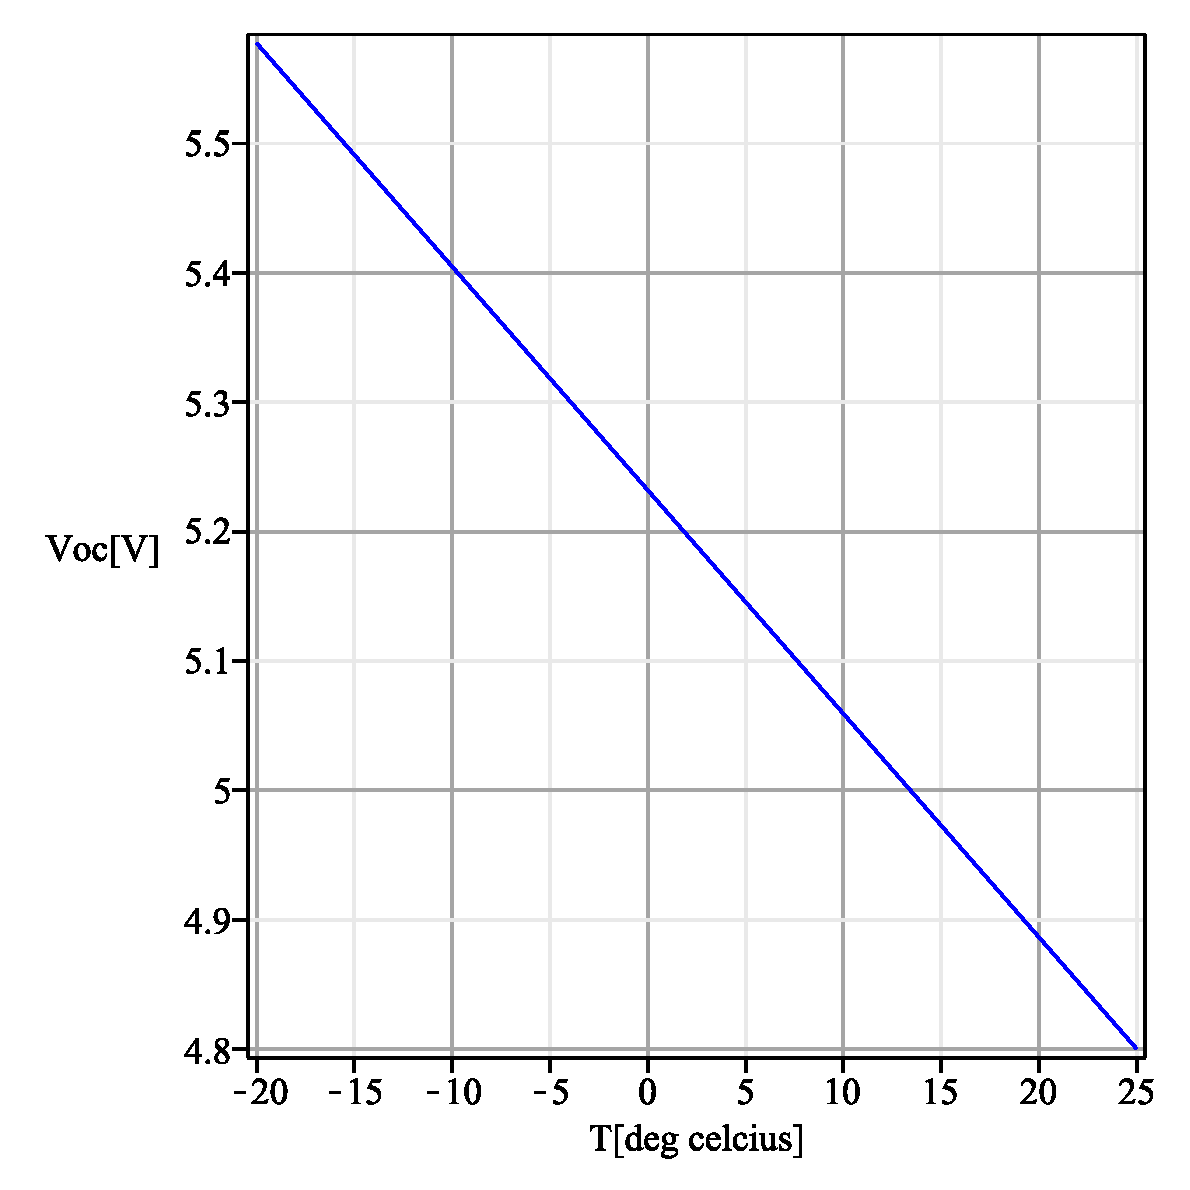
\includegraphics[height=0.28\textheight]{figures/fig_SA_Voc_temperature_dependence}
\end{minipage}
\caption{Temperature dependence on solar cell IV-characteristics}
\label{fig:SA_IV_temperature_dependence}
\end{figure}
%
%
\subsubsection*{Solar Incidence Angle}
The launch site of U-SPACE is near Kiruna at $67.5^{\circ}$ northern latitude. In summer solstice, at midday, the solar incidence angle, from local horizontal, is:

\begin{equation}
\begin{split}
\alpha _{sun}&=90^{\circ}-67.5^{\circ}+23,5^{\circ} =\\
\alpha _{sun}&=46^{\circ}
\end{split}
\end{equation}

The solar cell output current drops with the Kelly cosine function, shown in figure \ref{fig:KellyCosine}. To minimize power losses, due to inclined solar incidence, the optimal mounting position and angle of the solar panels must be considered.
%
\begin{figure}[H]
\centering
\includegraphics[scale=0.5]{figures/fig_KellyCosine}
\caption{Kelly cosine function showing how solar cell photo current depends on sun incidence angle}
\label{fig:KellyCosine}
\end{figure}
 %
\subsubsection*{Solar Array Shading}
Shading on the solar panels, for example caused by airship stabilizer structures or objects in the landscape, can cause a significant drop in the cell output voltage, as described in \cite[p. 165]{Mukund}. Bypass diodes can be used to partly mitigate this issue as well as using a \ac{MPPT} regulator. Otherwise it could be necessary to ensure that the airship structure cannot cast shadows on the panels and that the airship only fly above or away from landscape objects.
%
%
\subsection{Expected Performance}
%What are the expected performances of the subsystem, as related to the requirements above? (maybe including some margins)
%
\begin{table}[H]
\centering
\caption{Expected performance of the \ac{EPS}}
\label{tab:expected_performance}
\begin{minipage}{\textwidth}
\begin{tabular}{p{0.55\textwidth}p{0.35\textwidth}}
\hline
Power conversion efficiency(overall) & $80-90\%$\\
Power production(overall) & $9\,W < P_{avg} < 12.5\,W$\\
Battery capacity & $10.44\,Wh$\\
Mass & $\sim500-750\,g$\footnote{Depends on the chosen regulator design and system scaling}\\
\hline
\end{tabular}\par
\vspace{-0.75\skip\footins}
\renewcommand{\footnoterule}{}
\end{minipage}
\end{table}